\clearpage
\part*{Part VIII --- Factoring at size, and why elliptic curves fall first}
\addcontentsline{toc}{part}{Part VIII --- Factoring at size, and why elliptic curves fall first}

Parts I--VI factor with the textbook modular exponentiation: $4n$ Fourier adders per
multiplication and $2n$ counting qubits, verified exhaustively on numbers a laptop can simulate.
Part VII built the elliptic-curve discrete logarithm up to secp256k1. This part does the same for
RSA with the construction that holds the current record, Gidney's 2025 approximate residue
arithmetic \cite{ec:gidney25rsa}. It builds that construction at $n=1024$--$4096$ and puts the two
side by side, which is what the comparison ``ECDSA or RSA, which falls first'' actually needs.

\section{Gidney 2025, built}\label{rsa:sec:g25}

\subsection{What the circuit computes}

Shor's algorithm with Eker\aa{}--H\aa{}stad's short discrete logarithm needs $V=g^e\bmod N$ for an
exponent $e$ of $m=n/2+n/s$ qubits. With $e$ read $w_1$ bits at a time, $g^e$ is the exact integer
product of $W_1=\lceil m/w_1\rceil$ classical factors below $N$. So it is determined by its residues
modulo any set $P$ of small primes whose product $L$ exceeds $N^{W_1}$, and those residues can be
computed one prime at a time in registers of $\ell\approx21$ qubits. For each prime $p$:
\begin{enumerate}\setlength\itemsep{1pt}
\item \emph{loop1} adds looked-up discrete logarithms, $S_p=\sum_j\mathrm{dlog}_{g_p}M_{j,e_j}$, so the
multiplications become additions. It adds the \emph{difference} between this prime's table and the
previous one's, so computing prime $i$ and uncomputing prime $i-1$ is a single pass.
\item \emph{loop2} reduces $S_p$ modulo $p-1$ by binary long division.
\item \emph{loop3} computes $V_p=g_p^{S_p}\bmod p$ by windowed multiplications, measuring each
old result out instead of uncomputing it.
\item \emph{loop4} adds the top $f$ bits of $V_p u_p\bmod L\bmod N$ (the CRT basis) into the output.
\item \emph{unloop3} and \emph{unloop2} undo loops 3 and 2.
\end{enumerate}
Only the output accumulator is large, and it keeps just $f=33$ bits. It starts from a random mask,
which is what makes the truncation harmless to period finding. Every modular addition is a
subtraction with an extra borrow qubit that is cleared by measurement, and every lookup is
unloaded the same way.

\subsection{How it is checked}

The circuit (\texttt{rns.py}) is built on this package's machine from the same adders and lookups
as Part VII. A bit-exact integer model (\texttt{rns\_classical.reference}) replays every register:
the dlog sums, the long division, the windowed exponentiation, and the truncated, masked
accumulation. At $N=1003$ and $N=3127$ the circuit's output equals the model on every exponent,
with random masks and every ancilla checked clean. Separately, the model's approximation stays
within \cite{ec:gidney25rsa}'s deviation bound for every exponent at three toy moduli.

Knowing the answer, the whole output distribution can be checked too. The circuit is a permutation
on basis states, so its frequency distribution follows exactly from what it computes on each
exponent: Fourier transform each set of exponents the masked output register cannot tell apart,
and add the squares. For Eker\aa{}--H\aa{}stad at $N=241\times251$ with $s=2$, the residue system
has $@@toy_primes@@$ primes, none dividing $N$, and $L\bmod N=@@toy_lmod@@$; with $f=@@toy_f@@$ kept
bits the worst deviation is $@@toy_dev@@\%$ of $N$ (bound $@@toy_bound@@\%$). The textbook oracle's
distribution equals the closed form to $10^{-16}$. The approximate, masked one is at total variation
$@@toy_tvd@@$ from it and puts $@@toy_peak@@$ of its mass on the pairs that carry $90\%$ of the exact
distribution ($@@toy_epeak@@$ for the exact oracle): the same peaks. The masks trade one way: the
window of values they blur together must stay well below the period ($@@toy_window@@$ against
$@@toy_period@@$ here), and wider masks move the distance up. At smaller moduli
\cite{ec:gidney25rsa}'s bound $3|P|\ell/2^f$ exceeds one, and the approximation is visibly
unfaithful. That is a statement about toy sizes, not about $n=2048$, where the bound is
$\approx10^{-3}$.

\subsection{At size}

A shot is $|P|$ iterations of one prime's loops, plus a final loop1 and one merged phase repair
per exponent window. Every iteration is the same circuit up to its tables, and no gate count here
depends on the tables: lookups are unary or ANF, adders and comparisons have fixed width. The
bench builds the iteration for three different primes of a real random residue system, checks
that their counts agree, and multiplies by $|P|$:

\begin{center}\small
\begin{tabular}{rrrrrrr}
\toprule
$n$ & $|P|$ & one iteration & per shot & per factoring & \cite{ec:gidney25rsa} & qubits (paper)\\
\midrule
%%RSA_ROWS%%
\bottomrule
\end{tabular}
\end{center}

\noindent The Toffolis are executed ones (a measured repair counted at its probability), for
comparison with the paper, whose Table~5 does the same. Per factoring means per shot times the
expected $@@shots2048@@$ shots. The built counts are $@@over2048@@\%$ above the paper's at $n=2048$.
Part of the difference is that loop3's lookup repairs are done in place here, not merged into
unloop3's.

The qubit counts follow the paper's formula $m+3f+2\ell+\mathrm{len}\,m$ plus the adders'
scratch. The paper's own Table~5 is lower than its formula: $1\,399$ against
$@@tally_q2048@@$ at $n=2048$. Fed to the surface-code model, the paper's own inputs give its
headline, $@@g25_phys@@$ physical qubits and $@@g25_days@@$ days.

\section{ECDSA against RSA}\label{rsa:sec:gap}

\begin{center}
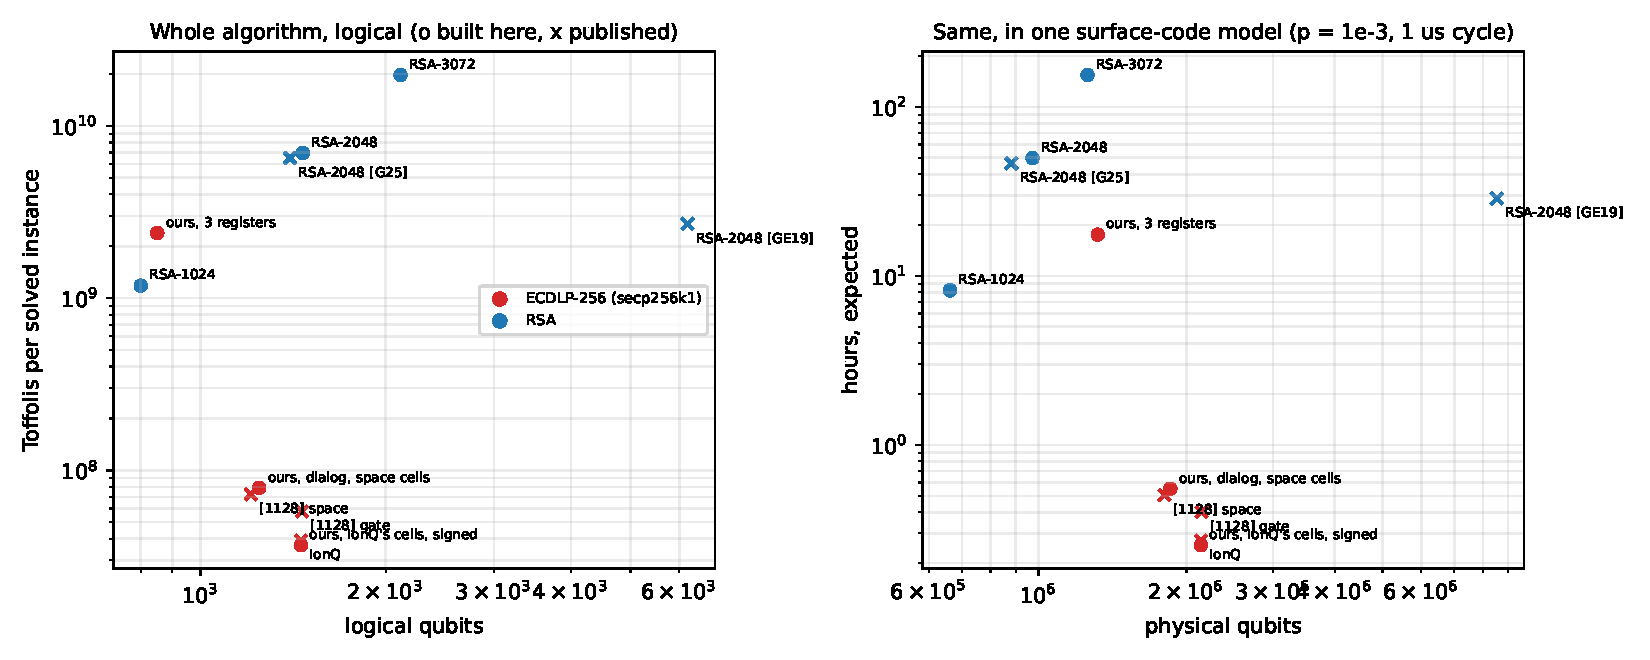
\includegraphics[width=\textwidth]{doc/figures/ecc_vs_rsa.pdf}
\end{center}

\begin{center}\small
\begin{tabular}{lrrrr}
\toprule
whole algorithm & logical qubits & Toffolis & physical qubits & days\\
\midrule
%%GAP_ROWS%%
\bottomrule
\end{tabular}
\end{center}

\noindent Every row uses the same physical model: $p=10^{-3}$, a $1\,\mu$s cycle, a $10\,\mu$s
reaction time, and six CCZ factories giving one CCZ every $25\,\mu$s. Runtime is the larger of
that throughput and the exact Toffoli depth times the reaction time; here the throughput always
binds. RSA's exponent register, idle except for its control windows, sits in cold yoked storage at
a third of the hot cost. The elliptic-curve circuits recycle their control qubits and keep
everything else busy. That is why RSA-2048 needs fewer \emph{physical} qubits than secp256k1 at a
comparable logical count, while taking $@@days_ratio@@$ times as long.

The logical qubit counts are close: $@@ecc_q@@$ for secp256k1 on IonQ's cells, $@@ecc_q_min@@$ on
the fewest-qubit cells, against $@@rsa_q@@$ for RSA-2048. The Toffoli counts are not: $@@ecc_t@@$
against $@@rsa_t@@$, a factor of $@@ratio@@$. Four things explain that factor.

\begin{enumerate}\setlength\itemsep{2pt}
\item \textbf{The numbers are eight times shorter.} Both algorithms spend their time on modular
arithmetic, whose cost grows at least as $n^2$ per group operation. An elliptic-curve group operation
needs an inversion, dozens of multiplications' worth. That buys a far smaller $n$ at the same
classical security: generic attacks on elliptic curves run in $2^{n/2}$, while factoring has the
sub-exponential number field sieve. Shor is polynomial in both cases, so the quantum cost follows
$n$, not the classical security level.
\item \textbf{One shot against nine.} The windowed ECDLP circuit succeeds in one run with high
probability. Eker\aa{}--H\aa{}stad with $s=8$ needs $s+1$ good shots, and masking and deviation cost
about $1\%$ more: $@@shots2048@@$ expected shots, each a full exponentiation.
\item \textbf{Approximation buys qubits, not Toffolis.} The residue arithmetic never holds an
$n$-bit number in superposition except the output's top $f$ bits. That is how RSA-2048 fits in
$@@rsa_q@@$ qubits, $0.7n$, while secp256k1 needs $4.9$--$8.7n$. The price is Toffolis: per prime,
loop1 reads all $W_1=214$ exponent windows, and there are $|P|\approx n W_1/\ell\approx21\,000$
primes, so a shot costs $\Theta(n\,m^2/(\ell\,w_1^2))$ lookups and additions of $\approx\ell$ bits.
\item \textbf{At equal classical security the gap widens.} RSA-2048 gives 112-bit security.
RSA-3072, the RSA size matched to secp256k1's 128 bits, costs $@@rsa3072_t@@$ Toffolis here,
$@@ratio3072@@\times$ the elliptic-curve count.
\end{enumerate}

\begin{center}
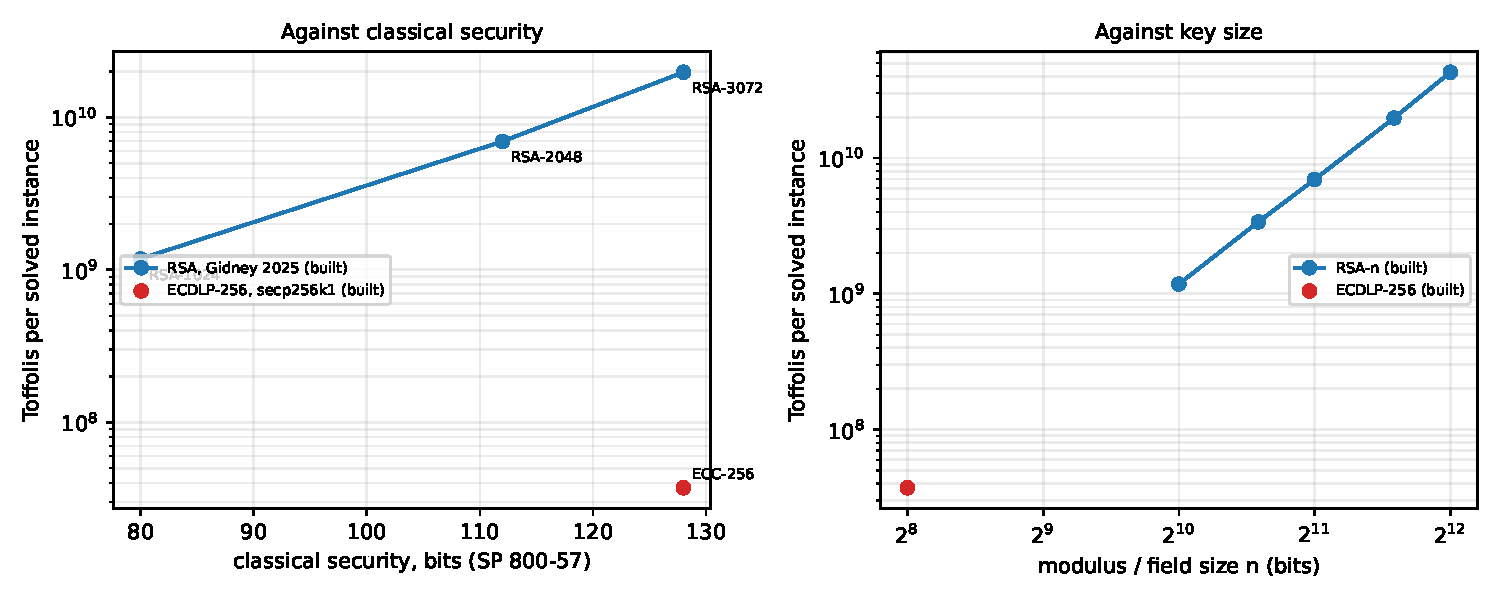
\includegraphics[width=0.62\textwidth]{doc/figures/security_vs_toffoli.pdf}
\end{center}

\begin{keybox}[title={The gap, in one line}]
At comparable qubit counts, breaking secp256k1 costs about $@@ratio@@$ times fewer Toffolis than
factoring RSA-2048, and $@@ratio3072@@$ times fewer than RSA-3072 at equal classical security. In
the same surface-code model that is $@@ecc_minutes@@$ minutes against $@@rsa_days@@$ days. Elliptic-curve keys
of today's sizes fall before RSA keys of today's sizes.
\end{keybox}
